\section{Governing Equations for Inviscid, Non-Equilibrium Flows}

Before reading the present section of the report, the reader is assumed to have prior knowledge about basic fluid dynamics equations and therefore all the governing equations that are involved in predicted the fluid movement and properties. Most of the governing equations are the same for the high temperature non-equilibrium flows as well but in addition to the species continuity equation which is assigned to the each of the species in the mixture. The continuity equation that is depicted in this current report will be termed as \emph{Global Continuity Equation} since the entire species has a single governing equation that can generalized to all the species that are present in the fluid in the flow field of interest.

\begin{figure}[ht]

\centering
  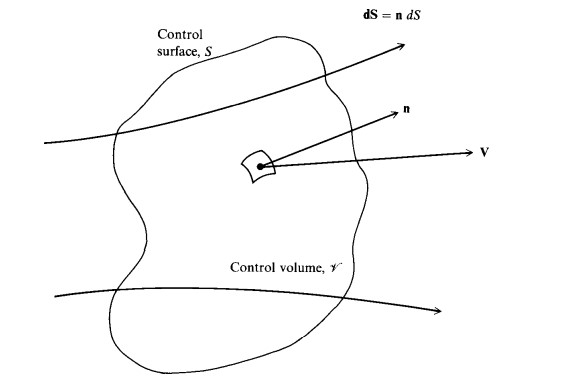
\includegraphics[width=0.5\linewidth]{images/control_volume.jpg}
  \caption{Finite-Control Volume fixed in space, with the flow moving through it}
  \label{fig:boat1}
\end{figure}

Let us the species continuity equation, Let us consider a fixed control volume as depicted in figure 2. The properties that are assumed are, The flowfield is inviscid, Non-Equilibrium in nature of a chemical reacting gas.

The mass of the species per unit volume is given by the below equation.
\[ \rho = \sum_{i}\rho_i  \ \]
\small where \[\rho_i\],  is the mass of species i per unit volume of the mixture.

Now let us try to predict the flow features by examining the figure 2, the mass flow of species i through the elemental surface
area dS is equation and equation2, where V is the local velocity vector and n is the unit normal vector and therefore the net mass flow of the species i out of the control volume is given by 

\vspace{3mm}
\[\iint\limits_s \rho_i.V.dS\]

\vspace{3mm}and therefore the mass of the individual species is considered to be 

\large \vspace{3mm} \[\iiint\limits_v \rho_i.dV\]
\vspace{3mm}

Now we must model the equations for the chemical reactions inside the control volume. The main things that should be noted are the net flux of species i that is passing through the surface, and the creation of extinction of the species that are present in the control volume as a result of chemical reactions. Not let W I be the local rate of change of density of each individual
species as a result of chemical reaction inside the control volume.

Hence the integral form of the governing equation turns out to be, which is very similar to the global continuity equation, 
\vspace{3mm}

\[\frac{\partial}{\partial t} \iiint\limits_v \rho_i.dV = -\iint\limits_s \rho_i.V.dS+\iiint\limits_v w_i.dV\] 

\vspace{3mm}
The differential form of the species continuity equation is given by, considering the flow to be inviscid, 

\large\vspace{3mm}\[\frac{\partial \rho_i }{\partial t} + \nabla .(\rho_i.V)\]
\vspace{3mm}
The above equation 5 and 6 are derived in the inviscid form, else additional term that is the transport of species and mass diffusion and the velocity would be the mass motion of each species i which is not the same throughout the fluid which finally contributes to the final fluid properties

If we consider the gas to be chemically reactive gas then there an additional term that gets involved that is weight of each species which is a component of the chemical rate equation. assuming the gas to Nitrogen Oxide (NO), the rate equation that is given assuming the dimensions of the given equation are said to in moles per unit volume per unit time and the molecular weight of each species is defined as mass of species i per mole of i, \vspace{3mm} 

 \large\[\frac{d[NO]}{dt} = k_{3fa}[NO][O_2]\] \vspace{3mm}

\large\[W_{NO} = M_{NO}.\frac{d[NO]}{dt}\]\vspace{3mm}

where M(NO) is the molecular weight of NO, therefore equation 6 can be written as \vspace{3mm}
Equation 8 \vspace{3mm}

where d(NO)/dt is obtained from the below equation
\vspace{3mm}
\large\[\frac{\partial \rho_NO }{\partial t} + \nabla .(\rho_{NO}.V)= M_{NO}.\frac{d[NO]}{dt}\]

An alternative form of species continuity equation, which the mixture of continuity equation and density equation, 

\vspace{3mm}
\large\[\rho[\frac{\partial c_i }{\partial t}+V.\nabla c_i] + c_i \frac{\partial c_i }{\partial t}+\nabla .(\rho.V) =w_i\]
The expanded form the equation is given below 
\vspace{3mm}
equation 11

if you observe the equation 11, the first two terms constitute the substantial derivative of ci. The second two terms result in zero from the global continuity equation and hence can be written in terms of mole mass ratio as well in equation 13,

\large\[\frac{D c_i}{D t}= \frac{w_i}{\rho}\]

\vspace{3mm}
\large\[\frac{D \eta_i}{D t}= \frac{w_i}{M_i \rho}\]

The primary notable quantities that are found in the above equations are c i and eeta 1 that is the governing terms that are present in the governing equations which are only influenced by finite chemical reaction terms or changes taking place within the element since the substantial derivative of a quantity is that is physically moving with time rate of change of that quantity.

Considering the non-equilibrium variable inside the substantial derivative is per unit mass of the mixture, then the right side of the equation of the conservation equation becomes is simple cause of chemical rate kinetics, using the above contrast the global continuity equation with respect to substantial derivative is given by 

\vspace{3mm}
\large\[\frac{D \eta_i}{D t}= w_i - \rho_i(\nabla . V)\]

In addition to the species continuity equation, the vibrational non-equilibrium is present, assuming the fluid element with fixed mass moves, the rate of change of vibrational energy is directly equal to the rate of molecular energy exchange inside the element and therefore the vibration energy relation of the moving element, where e vib is the local non-equilibrium value of vibrational energy per unit mass of gas, becomes,

\vspace{3mm}
\large\[\frac{D e_{vib}}{D t}= \frac{1}{\tau} (e^{eq}_{vib}-e_{vib})\]
\vspace{3mm}